\documentclass[fleqn]{beamer}

\usepackage{amsmath}
\usepackage{animate}
\usepackage{amsfonts}
\usepackage[mathscr]{eucal}
\usepackage{subcaption}
\usepackage{wrapfig}
\usepackage{graphicx}

\usepackage{fancyhdr}
\usepackage{pstricks}
\usepackage{pst-func}
\usepackage{pst-plot}
\usepackage[utf8x]{inputenc}
\usepackage[spanish]{babel}


\setbeamertemplate{navigation symbols}{}
\definecolor{UniBlue}{RGB}{83,121,170}
\setbeamercolor{frametitle}{fg=black,bg=white}
\setbeamercolor{title}{fg=black,bg=yellow!85!orange}
%\setbeamercolor{title}{fg=red,bg=yellow!90!blue}
\usetheme{Madrid}

\beamersetuncovermixins{\opaqueness<1>{25}}{\opaqueness<2->{15}}
\begin{document}

\title{OpenGL}
\author{Reynaldo Martell}
\date{\today} 

\begin{frame}
\titlepage
\end{frame}

\begin{frame}\frametitle{\rule{0mm}{10mm}\rule{5mm}{0mm} ¿Que es OpenGL?. }
OpenGL es un API que nos proporciona un gran conjunto de funciones con las que podemos usar para manipular gráficos e imágenes.
%\begin{figure}[H]
%	\centering
%	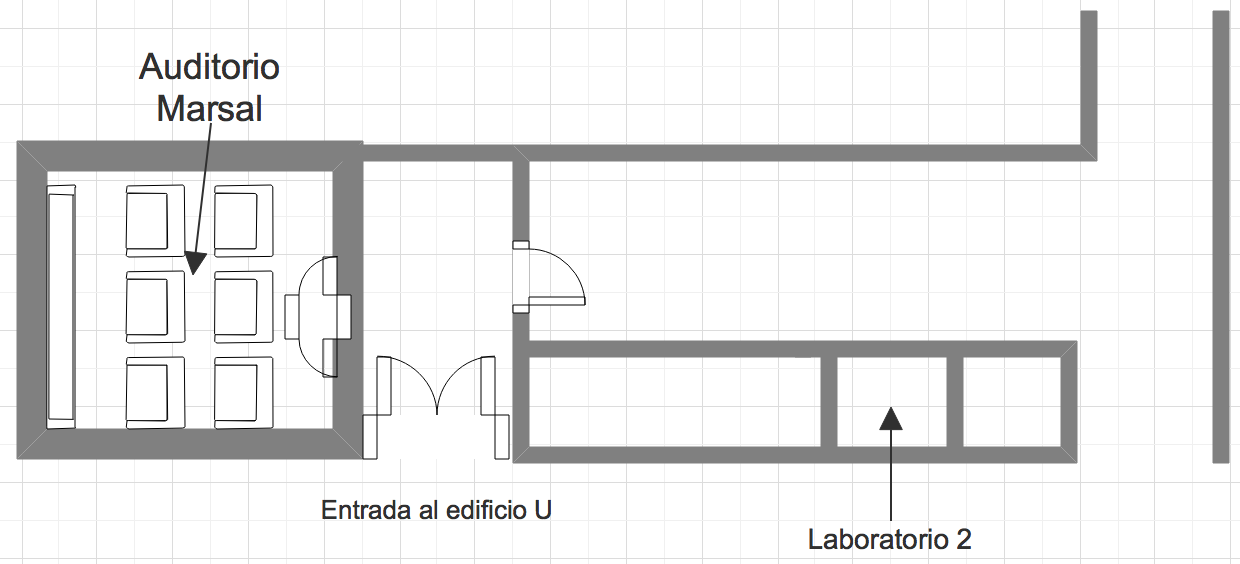
\includegraphics[width=1.0\textwidth]{images/mapa.png}
%	\label{mapa}
%\end{figure}
\end{frame}

\begin{frame}\frametitle{\rule{0mm}{10mm}\rule{5mm}{0mm} En el principio ... }
OpenGL es un API que nos proporciona un gran conjunto de funciones con las que podemos usar para manipular gráficos e imágenes.

\begin{itemize}
\item Los datos estaban representados solo por impulsos eléctricos que son invisibles al ojo.
\item Un método de visualización de estos datos tuvo que ser inventado, su nombre se llamó tarjetas perforadas.
\item Se necesitaba que su interpretación fuera legible.
\item La salida de las maquinas estaba lejos de ser óptima.
\end{itemize}

%\begin{figure}[H]
%	\centering
%	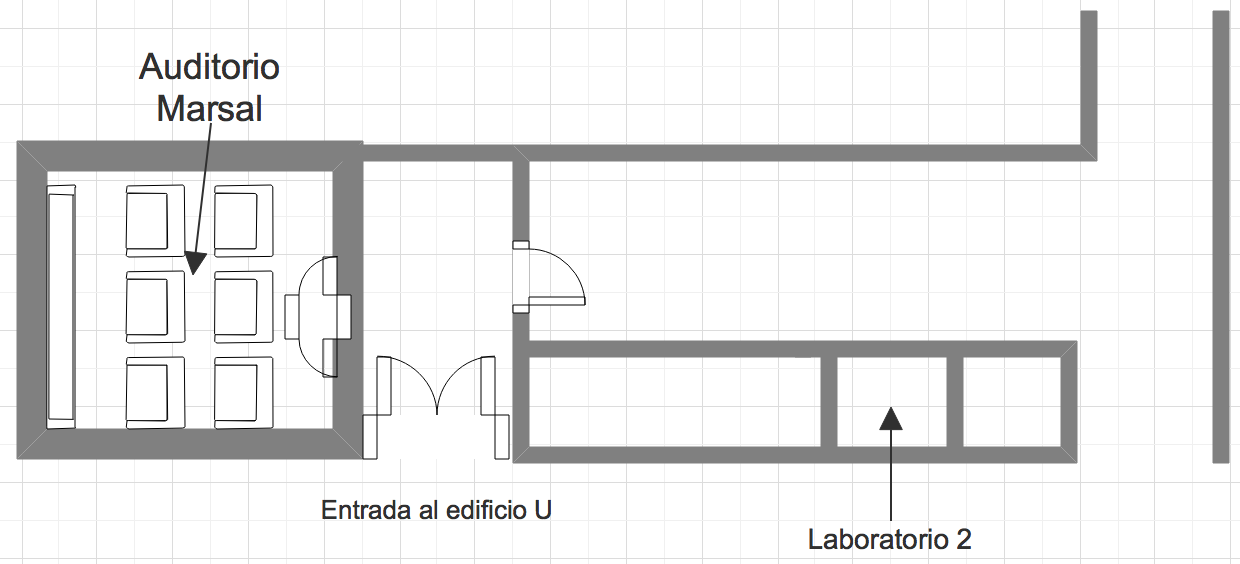
\includegraphics[width=1.0\textwidth]{images/mapa.png}
%	\label{mapa}
%\end{figure}
\end{frame}

\begin{frame}\frametitle{\rule{0mm}{10mm}\rule{5mm}{0mm} Las primeras interacciones. }

\begin{itemize}
\item En un inicio CRTs fue utilizado para mostrar el texto del estado de la computadora.
\item En 1961 Ivan Sutherland desarrollo un programa llamado Sketchpad.
\item Sketchpad permitía a los usuarios dibujar formas geométricas con una pluma de luz en tiempo real.
\begin{itemize}
\item Definió los gráficos por computadora.
\item Introdujo las interfaces de usuario.
\item Sentó las bases de la programación orientada a objetos.
\end{itemize}
\end{itemize}

\begin{figure}[H]
	\centering
	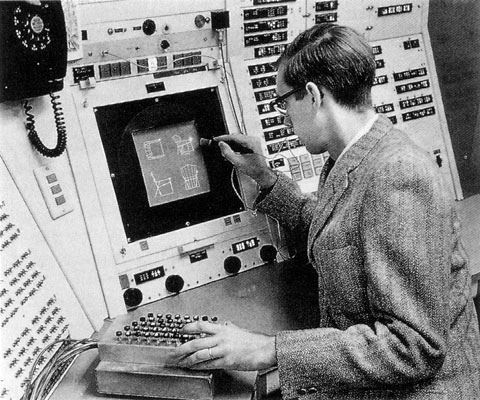
\includegraphics[width=0.35\textwidth]{images/Sketchpad.png}
	\label{mapa}
\end{figure}

%\begin{figure}[H]
%	\centering
%	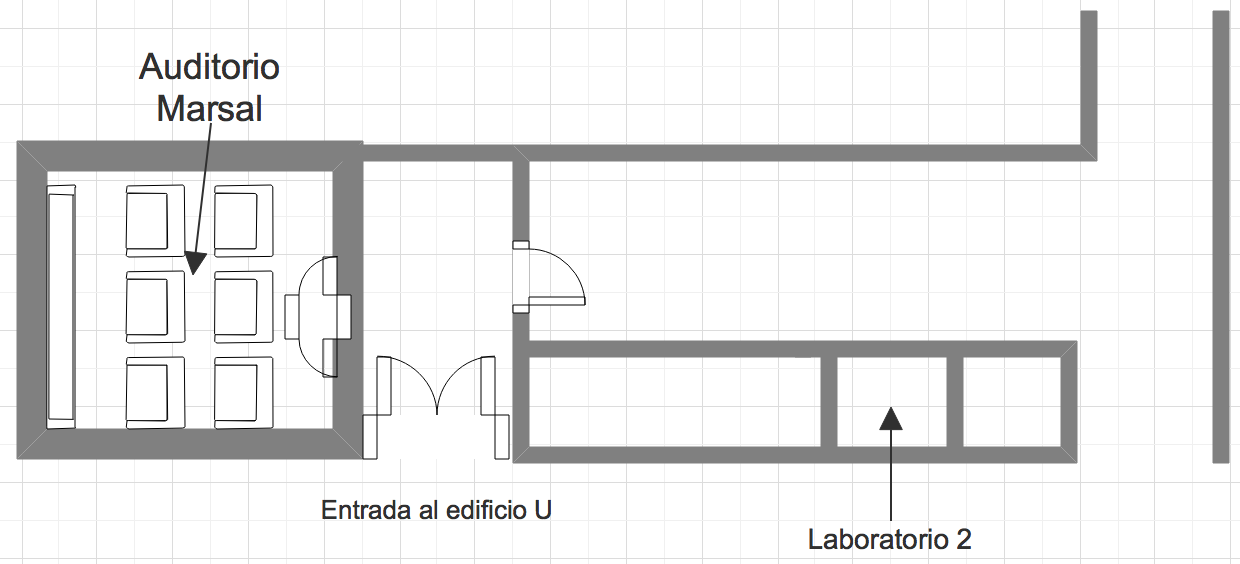
\includegraphics[width=1.0\textwidth]{images/mapa.png}
%	\label{mapa}
%\end{figure}
\end{frame}

\begin{frame}\frametitle{\rule{0mm}{10mm}\rule{5mm}{0mm} Las primeras interacciones. }

\begin{itemize}
\item En 1968 Ivan Sutherland y Bob Sproull diseñaron "La espada de Damocles".
\item Precursor de lo que ahora llamamos Realidad Virtual.
\end{itemize}

\begin{figure}[H]
	\centering
	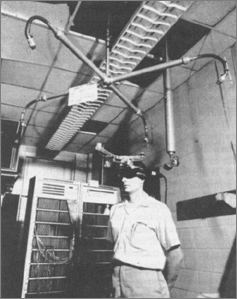
\includegraphics[width=0.35\textwidth]{images/Democles.png}
	\label{mapa}
\end{figure}
\end{frame}

\end{document}

